
\documentclass[handout]{beamer}  

%Smaller gap at between top and bottom of block when there are displayed equations
\addtobeamertemplate{block begin}{\setlength\abovedisplayskip{0pt}}
{\setlength{\belowdisplayskip}{0pt}}
\usepackage{appendixnumberbeamer}
\usepackage{lmodern}
\usepackage{setspace}
\linespread{1.2}
\usepackage{amssymb, amsmath, amsthm} 
\usepackage{rotating}
\usepackage{multirow}
\usepackage{graphicx}
\usepackage{synttree}
\usepackage{verbatim}
\usepackage{fancybox}
\usepackage{color}
\usepackage{tikz}
\usetikzlibrary{shapes,backgrounds}
\usepackage{hyperref}
\usetikzlibrary{trees}
\newcommand{\p}{\mathbb{P}}
\newcommand{\expect}{\mathbb{E}}


%\setbeamertemplate{blocks}[rounded][shadow=true] 
%gets rid of bottom navigation bars
\setbeamertemplate{footline}{
   \begin{beamercolorbox}[ht=4ex,leftskip=0.3cm,rightskip=0.3cm]{author in head/foot}
%    \usebeamercolor{UniBlue}
    \vspace{0.1cm}
    %\insertshorttitle \ - \insertdate 
    \hfill \insertframenumber / \inserttotalframenumber
   \end{beamercolorbox}
   \vspace*{0.1cm}
} 

%Put the math in red
\setbeamercolor{math text}{fg=red}

%gets rid of navigation symbols
\setbeamertemplate{navigation symbols}{}


%Include or exclude the notes?
%\setbeameroption{show notes}
\setbeameroption{hide notes}

\title[Econ 722]{Factor Models and High Dimensional Forecasting} 
\author[F. DiTraglia]{Francis J.\ DiTraglia}
\institute{University of Pennsylvania}
\date{Econ 722}


\begin{document} 
%%%%%%%%%%%%%%%%%%%%%%%%%%%%%%%%%%%%%%%%



\begin{frame}[plain]
	\titlepage 
	

\end{frame} 
%%%%%%%%%%%%%%%%%%%%%%%%%%%%%%%%%%%%%%%%
\begin{frame}
\frametitle{Survey Articles on Factor Models}

\begin{block}
	{Stock \& Watson (2010)}
	Best general overview of factor models and applications.
\end{block}

\begin{block}
	{Bai \& Ng (2008)}
Comprehensive review of large-sample results for high-dimensional factor models estimated via PCA.
\end{block}

\begin{block}
	{Stock \& Watson (2006)}
	Handbook chapter on forecasting with many predictors. One section is devoted to dynamic factor models.
\end{block}

\begin{block}
	{Breitung \& Eickmeyer (2006)}
	Brief overview with an application to Euro-area business cycles. 
\end{block}

\end{frame}
%%%%%%%%%%%%%%%%%%%%%%%%%%%%%%%%%%%%%%%%
\begin{frame}
	\frametitle{The Basic Idea}
	We're interested in settings with a large number of time series $N$ and a comparable number of time periods $T$. 
\end{frame}
%%%%%%%%%%%%%%%%%%%%%%%%%%%%%%%%%%%%%%%%
\begin{frame}[c]\frametitle{Example: Stock and Watson Dataset}
    

	\begin{figure}
		\centering
		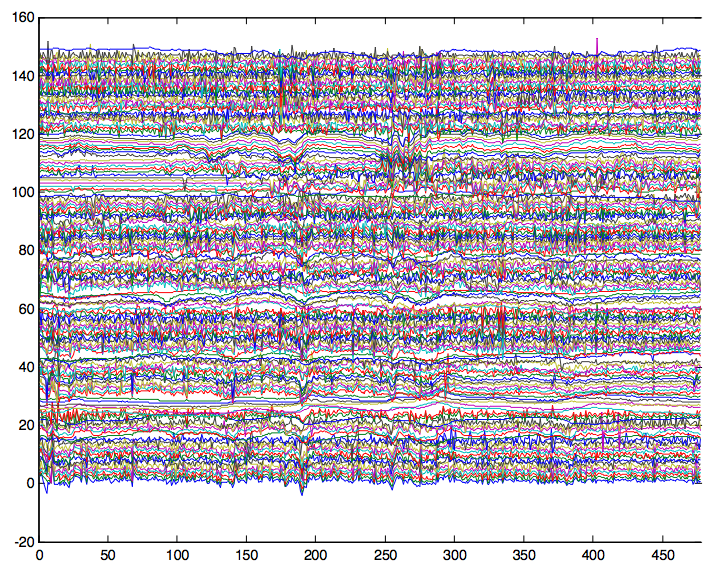
\includegraphics[scale = 0.3]{../img/stock_watson_dataset}
	\end{figure}
Monthly Macroeconomic Indicators: $N > 200, T >400$

\end{frame}

%%%%%%%%%%%%%%%%%%%%%%%%%%%%%%%%%%%%%%%%
\begin{frame}[c]\frametitle{Why Factor Models?}
   
\begin{enumerate}
	\item Factors could be intrinsically interesting if they arise from a theoretical model (e.g.\ Financial Economics)
	\item Many variables without running out of degrees of freedom\begin{itemize}
			\item More information could improve forecasts/macro analysis
			\item Mimic central banks ``looking at everything'' 
		\end{itemize}
	\item Eliminate measurement error and idiosyncratic shocks to provide more reliable information for policy
	\item ``Remain Agnostic about the Structure of the Economy''\begin{itemize}
		\item Advantages over SVARs: don't have to choose variables to control degrees of freedom, and can allow fewer underlying shocks than variables. 
	\end{itemize}
\end{enumerate}


\end{frame}
%%%%%%%%%%%%%%%%%%%%%%%%%%%%%%%%%%%%%%%%

\begin{frame}[c]\frametitle{Classical Factor Analysis Model}
    

  \alert{Assume that $X_t$ has been de-meaned\dots}

\vspace{1em}
$$\underset{(N\times 1)}{X_t} =  \Lambda \underset{(r\times 1)}{F_t} + \epsilon_t$$

\vspace{2em}

\small

$$
\left[ \begin{array}
	{c} F_t \\ \epsilon_t
\end{array}\right]
\overset{iid}{\sim} \mathcal{N}\left(
\left[ \begin{array}
	{c} 0\\ 0 
\end{array}\right],
\left[ \begin{array}
	{cc} I_r & 0\\
	0 & \Psi
\end{array}\right]\right)$$
\vspace{1em}

$\Lambda = $ matrix of factor loadings\\
$\Psi = $ diagonal matrix of idiosyncratic variances.
\end{frame}
%%%%%%%%%%%%%%%%%%%%%%%%%%%%%%%%%%%%%%%%
\begin{frame}
	\frametitle{Adding Time-Dependence}

\begin{eqnarray*}
	\underset{(N\times 1)}{X_t} &=&  \Lambda \underset{(r\times 1)}{F_t} + \epsilon_t \\ \\
	\underset{(r\times 1)}{F_t} &=& A_1 F_{t-1} + \hdots + A_p F_{t-p} + u_t \\ \\
	\left[ \begin{array}
	{c} u_t \\ \epsilon_t
\end{array}\right]
&\overset{iid}{\sim}& \mathcal{N}\left(
\left[ \begin{array}
	{c} 0\\ 0 
\end{array}\right],
\left[ \begin{array}
	{cc} I_r & 0\\
	0 & \Psi
\end{array}\right]\right)
\end{eqnarray*}	


\end{frame}
%%%%%%%%%%%%%%%%%%%%%%%%%%%%%%%%%%%%%%%%
\begin{frame}[c]\frametitle{Terminology}
 
\begin{description}
	\item[Static] $X_t$ depends only on $F_t$
	\item[Dynamic] $X_t$ depends on lags of $F_t$ as well
	\item[Exact] $\Psi$ is diagonal and $\epsilon_t$ independent over time
	\item[Approximate] Some cross-sectional \& temporal dependence in $\epsilon_t$
\end{description}

\vspace{1em}

\alert{The model I wrote down on the previous slide is sometimes called an ``exact, static factor model'' even though $F_t$ has dynamics.}

\end{frame}
%%%%%%%%%%%%%%%%%%%%%%%%%%%%%%%%%%%%%%%%

\begin{frame}
	\frametitle{Some Caveats}

\begin{enumerate}
	\item The difference between ``static'' and ``dynamic'' is unclear \begin{itemize}
		\item Can write dynamic model as a static one with more factors
		\item Static representation involves ``different'' factors, but we may not care: are the factors ``real'' or just a data summary?
	\end{itemize} 
	\item Not really possible to allow cross-sectional dependence in $\epsilon_t$ \begin{itemize}
		\item Unless the off-diagonal elements of $\Psi$ are close to zero we can't tell them apart from the common factors
		\item ``Approximate'' factor models basically assume conditions under which the off-diagonal elements of $\Psi$ are negligible
		\item Similarly, time series dependence in $\epsilon_t$ can't be very strong (stationary ARMA is ok)
	\end{itemize}
\end{enumerate}

\end{frame}
%%%%%%%%%%%%%%%%%%%%%%%%%%%%%%%%%%%%%%%%
\begin{frame}
	\frametitle{Methods of Estimation for Dynamic Factor Models}

	\begin{enumerate}
		\item Bayesian Estimation
		\item Maximum Likelihood: EM-Algorithm + Kalman Filter \begin{itemize}
			\item Watson \& Engle (1983)
			\item Ghahramani \& Hinton (1996)
			\item Jungbacker \& Koopman (2008)
			\item Doz, Giannone \& Reichlin (2012)
		\end{itemize}
		\item ``Nonparametric'' Estimation
			\begin{itemize}
				\item Just carry out PCA on $X$ and ignore the time-series element
				\item The first $r$ PCs are our estimates $\widehat{F}_t$
				\item Essentially treats $F_t$ as an $r$-dimensional \emph{parameter} to be estimated from an $N$-dimensional observation $X_t$
			\end{itemize}
	\end{enumerate}
\end{frame}

%%%%%%%%%%%%%%%%%%%%%%%%%%%%%%%%%%%%%%%%
\begin{frame}
\frametitle{Estimation by PCA}

\begin{block}
	{PCA Normalization}
		\begin{itemize}
			\item $F'F/T = I_r$ where $F = (F_1, \hdots, F_T)'$
			\item $\Lambda' \Lambda =\mbox{diag}(\mu_1, \hdots, \mu_r)$ where $\mu_1 \geq \mu_2 \geq \cdots \geq \mu_r$
		\end{itemize}
\end{block}
	
\begin{block}
	{Assumption I}
	Factors are \emph{pervasive}: $\Lambda' \Lambda/N \rightarrow D_\Lambda$ an $(r\times r)$ full rank matrix.
\end{block}

\begin{block}
	{Assumption II}
	$\max \;\mbox{e-value}\; E[\epsilon_t\epsilon_t']\leq c \leq \infty$ for all $N$.
\end{block}

\begin{block}
	{Upshot of the Assumptions}
If we average over the cross-section, the contribution from the factors persists and the contribution from the idiosyncratic terms disappears as $N\rightarrow \infty$.
\end{block}

\end{frame}
%%%%%%%%%%%%%%%%%%%%%%%%%%%%%%%%%%%%%%%%
\begin{frame}
	\frametitle{Key Result for PCA Estimation}
	Under the assumptions on the previous slide and some other technical conditions, the first $r$ PCs of $X$ consistently estimate the space spanned by the factors as $N,T \rightarrow \infty$.
\end{frame}
%%%%%%%%%%%%%%%%%%%%%%%%%%%%%%%%%%%%%%%%
\begin{frame}
	\frametitle{Doz, Giannone \& Reichlin (2012)}
\begin{block}
	{The arguments for the PCA approach\dots}
	\begin{itemize}
		\item Consistent estimation of factors under very weak assumptions 
		\item MLE is computationally infeasible for large $N$
	\end{itemize}
\end{block}

\begin{block}
	{\dots may be somewhat exaggerated.}
	\begin{itemize}
		\item EM-algorithm + Kalman Filter is \emph{very efficient} -- complexity depends on number of \emph{factors}, not number of series
		\item Treat exact, static factor model (the one I wrote out) as a mis-specified \emph{approximating model} (Quasi-MLE)
		\item Identical large-sample results as PC under similar assumptions, but better finite-sample properties and temporal smoothing
	\end{itemize}
\end{block}
\end{frame}
%%%%%%%%%%%%%%%%%%%%%%%%%%%%%%%%%%%%%%%%
%Is more data better? Problems with cross-sectional averaging
%%%%%%%%%%%%%%%%%%%%%%%%%%%%%%%%%%%%%%%%
\begin{frame}
	\frametitle{Choosing the Number of Factors}
If we use Likelihood-based or Bayesian estimation, we could try to resort to the familiar tools from earlier in the semester.There are a lot of parameters in factor models, however, so the asymptotic approximations (I'm looking at you, AIC) could be poor. 
\end{frame}
%%%%%%%%%%%%%%%%%%%%%%%%%%%%%%%%%%%%%%%%
\begin{frame}[c]\frametitle{Choosing the Number of Factors -- Scree Plot}
    
If we use PC estimation, we can look a something called a ``scree plot'' to help us decide how many PCs to include:
\begin{figure}
	\centering
	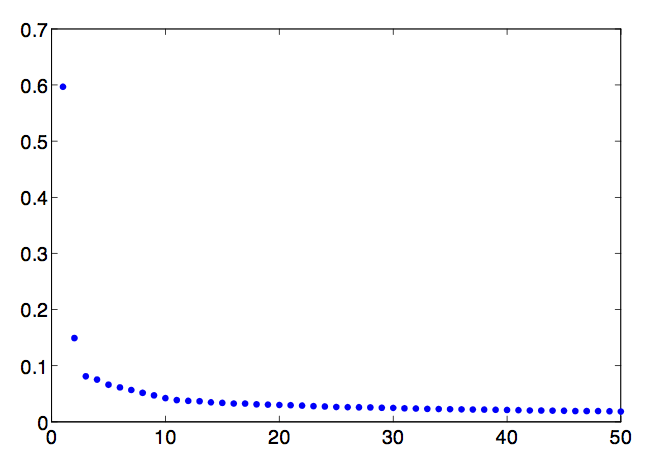
\includegraphics[scale =0.3]{../img/scree}
\end{figure}
This figure depicts the eigenvalues for an $N=1148, T = 252$ dataset of excess stock returns
\end{frame}
%%%%%%%%%%%%%%%%%%%%%%%%%%%%%%%%%%%%%%%%
\begin{frame}
	\frametitle{Choosing the Number of Factors -- Bai \& Ng (2002)}

Choose $r$ to minimize an information criterion:
$$IC(r) = \log V_r(\widehat{\Lambda}, \widehat{F}) + r \cdot g(N,T)$$
where
	$$V_r(\Lambda, F) = \frac{1}{NT}\sum_{t=1}^T (X_t - \Lambda F_t)'(X_t - \Lambda F_t)$$
and $g$ is a penalty function. The paper provides conditions on the penalty function that guarantee consistent estimation of the true number of factors. 
\end{frame}
%%%%%%%%%%%%%%%%%%%%%%%%%%%%%%%%%%%%%%%%
\begin{frame}
\frametitle{What Can We Do with Factors?}

Among other possibilities:
\begin{enumerate}
	\item Use them to construct Forecasts
	\item Use them as Instrumental Variables 
	\item Use them to ``Augment'' a VAR
\end{enumerate}

\vspace{1em}
\alert{We may not have time for the last two items this semester, so I've put them in the appendix to the slides below\dots}

\end{frame}

%%%%%%%%%%%%%%%%%%%%%%%%%%%%%%%%%%%%%%%%
\begin{frame}[c]\frametitle{Some Special Problems in High-dimensional Forecasting}
    

\begin{block}
	{Estimation Uncertainty} 
	We've already seen that OLS can perform very badly if the number of regressors is large relative to sample size.
\end{block}

\begin{block}
	{Best Subsets Infeasible}
	With more than 30 or so regressors, we can't check all subsets of predictors making classical model selection problematic.
\end{block}

\begin{block}
	{Noise Accumulation} 
	Large $N$ is supposed to help in factor models: averaging over the cross-section gives a consistent estimator of factor space. This can fail in practice, however, since it relies on the assumption that the factors are \emph{pervasive}. See Boivin \& Ng (2006).
\end{block}


\end{frame}
%%%%%%%%%%%%%%%%%%%%%%%%%%%%%%%%%%%%%%%%
\begin{frame}
	\frametitle{Main References}
	\begin{block}
		{Stock \& Watson (2006) -- ``Forecasting with Many Predictors''} Overview of high-dimesional forecasting with a review of forecast combination, factor models, and Bayesian approaches.
	\end{block}
	\begin{block}
		{Ng (2013) -- ``Variable Selection in Predictive Regressions''}
		Reviews and relates a number of shrinkage \& selection methods.
	\end{block}
	\begin{block}
		{Stock \& Watson (2012)}
		Examines a wide range of shrinkage procedures to see if they can improve on diffusion index forecasts.
	\end{block}
	\begin{block}
		{Kim \& Nelson (2013)}
		``Horse Race'' of various factor and shrinkage methods for forecasting.
	\end{block}
\end{frame}

%%%%%%%%%%%%%%%%%%%%%%%%%%%%%%%%%%%%%%%%
\begin{frame}[c]\frametitle{Diffusion Index Forecasting -- Stock \& Watson (2002a,b)}
 \framesubtitle{JASA paper has the theory, JBES paper has macro forecasting example.}

\begin{block}
	{Basic Setup}
	Forecast scalar time series $y_{t+1}$ using $N$-dimensional collection of time series $X_t$ where we observe periods $t = 1, \hdots, T$.
\end{block}

\begin{block}
	{Assumption}
	Static representation of Dynamic Factor Model:
	\begin{eqnarray*}
		y_{t}&\alert{=}& \beta' F_t + \gamma(L)y_t + \epsilon_{t+1}\\
		\alert{X_t} &\alert{=}& \alert{\Lambda F_t + e_t}
	\end{eqnarray*}
\end{block}

\begin{block}
	{``Direct'' Multistep Ahead Forecasts}
	``Iterated'' forecast would be linear in $F_t$, $y_t$ and lags:
	$$y_{t+h}^h = \alpha_h + \beta_h(L)F_t +  \gamma_h(L)y_t + \epsilon^h_{t+h}$$
\end{block}
\end{frame}
%%%%%%%%%%%%%%%%%%%%%%%%%%%%%%%%%%%%%%%%

\begin{frame}
\begin{center}
	\Huge This is really just PCR
\end{center}
\end{frame}

%%%%%%%%%%%%%%%%%%%%%%%%%%%%%%%%%%%%%%%%
\begin{frame}[c]\frametitle{Diffusion Index Forecasting -- Stock \& Watson (2002a,b)}
    
    \begin{block}
    	{Estimation Procedure}
    	\begin{enumerate}
    		\item Data Pre-processing
    			\begin{enumerate}
    			\item Transform all series to stationarity (logs or first difference)
				\item Center and standardize all series
				\item Remove outliers (ten times IQR from median)
				\item Optionally augment $X_t$ with lags
    			\end{enumerate}
    		\item Estimate the Factors
    			\begin{itemize}
    				\item No missing observations: PCA on $X_t$ to estimate $\widehat{F}_t$ 
		\item Missing observations/Mixed-frequency: EM-algorithm
    			\end{itemize}
    		\item Fit the Forecasting Regression
    		\begin{itemize}
    			\item Regress $y_{t}$ on a constant and lags of $\widehat{F}_t$ and $y_t$ to estimate the parameters of the ``Direct'' multistep forecasting regression.
    		\end{itemize}
    	\end{enumerate}
    \end{block}


\end{frame}
%%%%%%%%%%%%%%%%%%%%%%%%%%%%%%%%%%%%%%%%
\begin{frame}[c]\frametitle{Diffusion Index Forecasting -- Stock \& Watson (2002b)}
    
\alert{Recall from above that, under certain assumptions, PCA consistently estimates the space spanned by the factors. Broadly similar assumptions are at work here.}

\vspace{2em}

\begin{block}
	{Main Theoretical Result}
	Moment restrictions on $(\epsilon, e, F)$ plus a ``rank condition'' on $\Lambda$ imply that the MSE of the procedure on the previous slide converges to that of the infeasible optimal procedure, provided that  $N,T \rightarrow \infty$.
\end{block}

\end{frame}

%%%%%%%%%%%%%%%%%%%%%%%%%%%%%%%%%%%%%%%%
\begin{frame}[c]\frametitle{Diffusion Index Forecasting -- Stock \& Watson (2002a)}
    
\begin{block}
	{Forecasting Experiment}
	\begin{itemize}
		\item Simulated real-time forecasting of eight monthly macro variables from 1959:1 to 1998:12
		\item Forecasting Horizons: 6, 12, and 24 months
		\item ``Training Period'' 1959:1 through 1970:1
		\item Predict $h$-steps ahead out-of-sample, roll and re-estimate.
		\item BIC to select lags and \# of Factors in forecasting regression
		\item Compare Diffusion Index Forecasts to Benchmark
			\begin{itemize}
				\item AR only
				\item Factors only
				\item AR + Factors
			\end{itemize}
	\end{itemize}
\end{block}

\end{frame}
%%%%%%%%%%%%%%%%%%%%%%%%%%%%%%%%%%%%%%%%
\begin{frame}[c]\frametitle{Diffusion Index Forecasting -- Stock \& Watson (2002a)}
   \begin{block}
   	{Empirical Results}
   	\begin{itemize}
   		\item Factors provide a substantial improvement over benchmark forecasts in terms of MSPE
   		\item Six factors explain 39\% of the variance in the 215 series; twelve explain 53\%  
   		\item Using all 215 series tends to work better than restricting to balanced panel of 149 (PCA estimation)
   		\item Augmenting $X_t$ with lags isn't helpful
   	\end{itemize}
   \end{block}


\end{frame}

%%%%%%%%%%%%%%%%%%%%%%%%%%%%%%%%%%%%%%%%
% \begin{frame}
% 	\frametitle{Another Line of Research on Factor Models}

% The assumption of a factor structure sure is convenient, but how does it relate to other kinds of assumptions we're more familiar with? (e.g.\ everything follows a VAR). Does this structure come out of our economic models, or is it just an assumption of convenience? I haven't seen much work on this, but it seems important to me. Two recent papers that consider questions along these lines: Onatski and Ruge (2012), Dufour \& Stevanovic
% \end{frame}

%%%%%%%%%%%%%%%%%%%%%%%%%%%%%%%%%%%%%%%%
\begin{frame}[c]\frametitle{What about Ridge and Lasso?}
    
 \begin{block}
 	{Basic Idea}
 	Diffusion index forecasts are really just PCR. Why not try Ridge or Lasso with all predictors rather than estimating factors?
 \end{block}

 \begin{block}
 	{De Mol, Giannone \& Reichlin (2008)}
 	\begin{itemize}
 		\item Compare PCA-based factor forecasts to Ridge and Lasso
 		\item In a small out-of-sample experiment, Ridge and Lasso with appropriate penalty parameters give results comparable to diffusion index.
 		\item Analyze asymptotics of Ridge under assumptions typically used to justify PCA
 	\end{itemize}
 
 \end{block}



\end{frame}
%%%%%%%%%%%%%%%%%%%%%%%%%%%%%%%%%%%%%%%%
\begin{frame}[c]\frametitle{Other Ways of Extracting Factors}
    
    \begin{block}
    	{Sparse PCA}
    	Add a Lasso-type penalty to the ``regression'' formulation of PCA: encourage the factors to load on small number of variables.
    \end{block}

    \begin{block}
    	{Independent Components Analysis (ICA)}
    	Extract factors that maximize non-Gaussianity
    \end{block}

\vspace{1em}

\alert{Both of these are considered in Kim \& Swanson (2014) and seem to work very well when combined with second-stage shrinkage.}


\end{frame}
%%%%%%%%%%%%%%%%%%%%%%%%%%%%%%%%%%%%%%%%
\begin{frame}[c]\frametitle{To Target or Not to Target?}
    
    \begin{block}
    	{Problem with PCA and Friends}
    	Completely ignores $Y$ in constructing the factors! Should we take the forecast target into account when extracting factors?
	\end{block}

\begin{block}
	{Some References}
	\begin{itemize}
		\item Bai \& Ng (2008) -- Forecasting Economic Time Series Using Targeted Predictors
		\item Kelly \& Pruitt (2012) -- The Three-pass Regression Filter 
	\end{itemize}
\end{block}

\end{frame}

%%%%%%%%%%%%%%%%%%%%%%%%%%%%%%%%%%%%%%%%
\begin{frame}[c]\frametitle{Partial Least Squares (PLS)}

\begin{block}
	{As an Optimization Problem}
	Construct a sequence of linear combinations of $X$ that solve
	$$\underset{\alpha}{\max} \; Corr^2(\textbf{y}, X\alpha)Var(X\alpha)$$
subject to $||\alpha ||=1$ and the constraint that each PLS ``factor'' is orthogonal to the preceding ones.
\end{block}

\begin{block}
	{As a Probabilistic Model}
	``Shared'' factor $F_t$ and $X$-specific factor $Z_t$
	\begin{eqnarray*}
		Y_t &=& \mu_Y + \Lambda_Y F_t + \epsilon_t\\
		X_t &=& \mu_X + \Lambda_X F_t + \Pi Z_t + u_t
	\end{eqnarray*}
	where $F_t \perp Z_t$
\end{block}

\end{frame}

%%%%%%%%%%%%%%%%%%%%%%%%%%%%%%%%%%%%%%%%

\begin{frame}[c]\frametitle{Bootstrap Aggregation -- ``Bagging''}
    
\begin{block}
	{Bagging Algorithm}
	\begin{enumerate}
		\item Make a bootstrap draw  
		\item Carry out selection/shrinkage/estimation using boostrap data
		\item Use estimated parameters from to construct a forecast $\widehat{y}_{T+h}^{(b)}$
		\item Repeat for $b = 1, \hdots, B$
		\item Average to get ``Bagged'' Forecast: $\widehat{y}_{T+h}^{(Bag)} = \frac{1}{B}\sum_{b=1}^B \widehat{y}_{T+h}^{(b)}$
	\end{enumerate}
\end{block}

\begin{block}
	{Details}
	\begin{itemize}
		\item If the data are dependent, need block bootstrap.
		\item In step 3, we forecast using the \emph{parameters} estimated from the bootstrap data but the \emph{predictors} from the \emph{real} dataset.
	\end{itemize}
\end{block}

\end{frame}
%%%%%%%%%%%%%%%%%%%%%%%%%%%%%%%%%%%%%%%%
\begin{frame}[c]\frametitle{Bootstrap Aggregation -- ``Bagging''}

\begin{block}
 	{Why Bagging?}
 		\begin{itemize}
 			\item Aims to reduce the forecast error of ``unstable'' procedures such as variable selection of Lasso, by reducing their variance.
 			\item Completely portable: you can bag \emph{anything} provided you have an appropriate way to carry out the bootstrap.
 			\item May provide a way of attacking the problem of inference post-model selection. See Efron (JASA, \emph{Forthcoming}) ``Estimation and Accuracy after Model Selection''
 		\end{itemize}
 \end{block} 


\end{frame}
%%%%%%%%%%%%%%%%%%%%%%%%%%%%%%%%%%%%%%%%
\begin{frame}
	\frametitle{Bagging in Economics}
	\begin{block}
		{Inoue \& Killian (2008, JASA)}
		Compares performance of bagged ``pre-test'' estimator (variable selection via a t-test) to other methods of forecasting US Inflation. Bagging is carried out via a block bootstrap.
	\end{block}
	\begin{block}
		{Stock \& Watson (2012)}
		Among other shrinkage procedures, they consider a large-sample approximation to bagging pre-test estimators that doesn't require making bootstrap draws.
	\end{block}
	\begin{block}
		{Other Papers That Use Bagging}
		\begin{itemize}
			\item Hillebrand \& Medeiros (2010): Realized Volatility Forecasts
			\item Hillebrand et al (2012): Forecasting the Equity Premium
			\item \alert{Kim and Swanson (2013)}
		\end{itemize}
	\end{block}
\end{frame}
%%%%%%%%%%%%%%%%%%%%%%%%%%%%%%%%%%%%%%%%
\begin{frame}
	\frametitle{Boosting}
	\begin{block}
		{Ensemble Methods}
		Machine learning term for ``non-Bayesian model averaging''
	\end{block}
	\begin{block}
		{What is Boosting?}
		\begin{itemize}
			\item Combine large number of ``weak learners'' (i.e.\ crappy predictive models) so that the \emph{ensemble} predicts well.
			\item Explicitly designed around predictive loss
			\item Arbitrarily improve in-sample fit of arbitrarily the weak learners!
		\end{itemize}
	\end{block}
	\begin{block}
		{Book-Length Treatment}
		Shapire \& Freund (2012) -- \emph{Boosting: Foundations and Algorithms}
	\end{block}
\end{frame}

%%%%%%%%%%%%%%%%%%%%%%%%%%%%%%%%%%%%%%%%
\begin{frame}[c]\frametitle{Boosting}
    

 \begin{block}
 	{Bai \& Ng (2009) -- Boosting Diffusion Indices}
 	Use boosting to select which lags of factors to include in a forecasting regression estimated following PCA. 
 \end{block}

 \begin{block}
 	{Buchen \& Wohlrabe (2011) -- Is Boosting a Viable Alternative?}
 	Boosting performs well compared to other methods in the example from the 2006 Stock \& Watson Handbook Chapter.
 \end{block}

 \begin{block}
 	{Ng (2014) -- Boosting Recessions}
 \end{block}
\end{frame}
%%%%%%%%%%%%%%%%%%%%%%%%%%%%%%%%%%%%%%%%
\appendix
\begin{frame}
  \begin{center}
  \Huge Appendix
\end{center}
\end{frame}

%%%%%%%%%%%%%%%%%%%%%%%%%%%%%%%%%%%%%%%%
\begin{frame}[c]\frametitle{Factors as Instruments -- Bai \& Ng (2010)}
\begin{block}
   	{Endogenous Regressors $x_t$}
$$y_t = x_t' \beta + \epsilon_t \quad \quad E[x_t\epsilon_t] \neq 0 $$
\end{block}   

 \begin{block}
 	{Unobserved Variables $F_t$ are Strong IVs}
$$\underset{(k\times 1)}{x_t} = \Psi'\underset{(r\times 1)}{F_t} + u_t \quad \quad E[F_t \epsilon_t] = 0$$
 \end{block}

\begin{block}
	{Observe Large Panel $(z_{1t}, \hdots, z_{Nt})$}
		$$z_{it} = \lambda_i' F_t + e_{it}$$
\end{block}

\end{frame}

%%%%%%%%%%%%%%%%%%%%%%%%%%%%%%%%%%%%%%%%

\begin{frame}[c]\frametitle{Factors as Instruments -- Bai \& Ng (2010)}

\small

$$\boxed{
	y_t = x_t' \beta + \epsilon_t, \quad \quad
	x_t = \Psi'F_t + u_t, \quad \quad
	z_{it} = \lambda_i' F_t + e_{it}
}$$
\vspace{1em}

\begin{block}
	{Procedure}
	\begin{enumerate}
		\item Calculate the PCs of Z
		\item Calculate $\widetilde{F}_t$ using the first $r$ PCs of Z
		\item Use $\widetilde{F}_t$ in place of $F_t$ for IV estimation
	\end{enumerate}
\end{block}

\begin{block}
	{Main Result}
	Under certain assumptions, as $(N,T) \rightarrow \infty$ ``estimation and inference can proceed as though $F_t$ were known.'' The resulting estimator is consistent and asymptotically normal.
\end{block}

\normalsize

\end{frame}
%%%%%%%%%%%%%%%%%%%%%%%%%%%%%%%%%%%%%%%%
\begin{frame}[c]\frametitle{Factors as Instruments -- Bai \& Ng (2010)}
    
\begin{block}
	{Why Might This be Helpful?}
	\begin{enumerate}
		\item Avoid many instruments bias
		\item Avoid bias from irrelevant instruments
		\item Allow more observed instruments $z_{it}$ than sample size $T$
		\item Provided that $\sqrt{T}/N \rightarrow 0$, all of the observed instruments $z_{it}$ can be \emph{endogenous} as long as $F_t$ is exogenous
	\end{enumerate}
\end{block}

\end{frame}
%%%%%%%%%%%%%%%%%%%%%%%%%%%%%%%%%%%%%%%%
\begin{frame}[c]\frametitle{FAVARs -- Bernanke, Boivin \& Eliasz (2005)}
   
   \begin{block}
    	{Two Problems with Structural VARs}
    	\begin{enumerate}
    		\item Number of parameters is \emph{quadratic} in the number of variables. Unrestricted VAR infeasible unless $T$ is large relative to $N$.\begin{itemize}
    			\item You've studied one solution to this problem already this semester: Bayesian Estimation with informative priors 
    		\end{itemize}
    		\item To keep estimation tractable we typically use a small number of variables, but then the VAR innovations ``might not span the space of structural shocks.''
    	\end{enumerate}
    \end{block} 


\end{frame}

%%%%%%%%%%%%%%%%%%%%%%%%%%%%%%%%%%%%%%%%
\begin{frame}[c]\frametitle{FAVARs -- Bernanke, Boivin \& Eliasz (2005)}

\begin{block}{Factor-Augmented VAR Model}
	\begin{eqnarray*}
		\left[\begin{array}
			{c} Y_t \\ F_t
		\end{array} \right] &=& \Phi(L)\left[\begin{array}
			{c} F_{t-1} \\ Y_{t-1}
		\end{array} \right] + v_t\\ \\
		X_t &=& \Lambda^f F_t + \Lambda^y Y_t + e_t
	\end{eqnarray*}

\vspace{2em}

\small
$\underset{(M\times 1)}{Y_t} = $  observable variables that ``drive dynamics of the economy''\\ \vspace{1em}
$\underset{(K\times 1)}{F_t} = $ Small \# of unobserved factors: ``additional information''\\ \vspace{1em}
$\underset{(N\times 1)}{X_t} = $ Large \# of observed ``informational time series''
\end{block}

\end{frame}
%%%%%%%%%%%%%%%%%%%%%%%%%%%%%%%%%%%%%%%%
\begin{frame}[c]\frametitle{FAVARs -- Bernanke, Boivin \& Eliasz (2005)}

\small
$$\boxed{\quad \left[\begin{array}
			{c} Y_t \\ F_t
		\end{array} \right] = \Phi(L)\left[\begin{array}
			{c} F_{t-1} \\ Y_{t-1}
		\end{array} \right] + v_t \quad \quad \quad \quad
		 X_t = \Lambda^f F_t + \Lambda^y Y_t + e_t \quad}$$
\normalsize

\begin{block}{Consider Two Estimation Procedures}
	\begin{enumerate}
		\item Two-step Procedure:\begin{itemize}
			\item Estimate space spanned by factors using first $K + M$ PCs of $X$
			\item Estimate VAR with $\widehat{F}_t$ in place of $F_t$
		\end{itemize}
		\item Full Bayes (Gibbs Sampler)
	\end{enumerate}
\end{block}

\begin{block}{Empirical Application}
Additional information contained in FVAR is ``important to properly identify the monetary transmission mechanism.''
\end{block}
\end{frame}
%%%%%%%%%%%%%%%%%%%%%%%%%%%%%%%%%%%%%%%%
\end{document}
